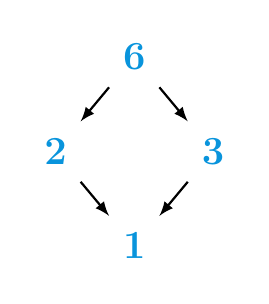
\begin{tikzpicture}[>=latex]

% --- Stijldefinities ---
\tikzset{
    getal/.style={
        text=cyan!80!blue, 
        font=\Large\bfseries, 
        inner sep=6pt
    },
    pijl/.style={
        ->,
        >=latex,
        thick,
        draw=black, % Past mooi bij de kleur van de getallen
        shorten >=0.1pt,      % Zorgt dat de pijl het getal niet snijdt
        shorten <=0.1pt
    }
}

% --- Knooppunten (Nodes) ---
\node[getal] (n6) at (0, 2.4) {6};
\node[getal] (n2) at (-1, 1.2) {2};
\node[getal] (n3) at (1, 1.2)  {3};
\node[getal] (n1) at (0, 0)   {1};

% --- Pijlen ---
\draw[pijl] (n6) -- (n3);
\draw[pijl] (n6) -- (n2);
\draw[pijl] (n2) -- (n1);
\draw[pijl] (n3) -- (n1);
\end{tikzpicture}